% !TeX program = xelatex
% AI for Theological Inquiry — "Packaging: from CLI to chatbot" segment deck.
% A ~30–40 min module, not a full session: drop it at the end of the Week 4 RAG
% lab, or use it to open the Week 11 build sprint. Build: xelatex packaging_chatbot.tex (twice).
% beamer-slides house preamble.
% Copy into a new deck and edit \deckauthor / \deckemail / \deckdate / colors.
% Build: xelatex deck.tex (run twice). See ../SKILL.md for the full house style.
\documentclass[aspectratio=169,11pt]{beamer}

\usetheme{metropolis}
\usepackage{fontspec}
\usepackage{graphicx}
\usepackage{tikz}
\usetikzlibrary{arrows.meta,positioning,shapes.geometric,fit,shadows}
\usepackage{tcolorbox}
\tcbuselibrary{skins,breakable}
\usepackage{fontawesome5}
\usepackage{listings}
\usepackage{booktabs}
\usepackage{array}

% ---------------------------------------------------------------- palette
% Placeholder professional navy/accent palette — swap for the exact ANL/ALCF
% brand hex values if you have the brand guide; do not present these as
% "official" institutional colors.
\definecolor{labnavy}{RGB}{18,42,73}
\definecolor{labink}{RGB}{40,44,52}
\definecolor{accentgold}{RGB}{223,161,54}
\definecolor{accentteal}{RGB}{0,137,123}
\definecolor{accentblue}{RGB}{41,98,168}
\definecolor{lightgray}{RGB}{245,246,248}
\definecolor{midgray}{RGB}{110,118,129}

% Hard rule: background is always white.
\setbeamercolor{background canvas}{bg=white}
\setbeamercolor{palette primary}{bg=labnavy,fg=white}
\setbeamercolor{frametitle}{bg=labnavy,fg=white}
\setbeamercolor{progress bar}{fg=accentteal,bg=lightgray}
\setbeamercolor{normal text}{fg=labink}
\setbeamercolor{alerted text}{fg=accentgold}
\setbeamercolor{footline}{fg=midgray}
\setbeamerfont{footline}{size=\tiny}

% Tighter default itemize indentation (see SKILL.md Gotchas — do NOT pass
% [leftmargin=...] to Beamer's itemize, that slot is for overlay specs).
\setlength{\leftmargini}{14pt}

% ---------------------------------------------------------------- deck metadata
% Fill these in per-deck. Email + date are a hard rule on the title page.
\newcommand{\deckauthor}{Huihuo Zheng}
\newcommand{\deckemail}{huihuo.zheng@wheaton.edu}
\newcommand{\deckinstitute}{Wheaton College}
% \date{...} still needs to be called explicitly in the document, e.g. \date{\today}

% ---------------------------------------------------------------- logo
% Looks for a real logo file first; falls back to a plain text lockup rather
% than fabricating the institutional mark. Put the real file at
% logos/argonne_logo.pdf (or .png) next to the deck, or point this at a
% shared assets/logos/ path.
% Drop a real logo at logos/wheaton_logo.pdf (or .png) to use it; otherwise
% this falls back to a plain text lockup rather than fabricating the mark.
\newcommand{\decklogo}[1][0.16\textwidth]{%
  \IfFileExists{logos/wheaton_logo.pdf}%
    {
\includegraphics[width=#1]{logos/wheaton_logo.pdf}}%
    {\IfFileExists{logos/wheaton_logo.png}%
      {
\includegraphics[width=#1]{logos/wheaton_logo.png}}%
      {\begin{minipage}{#1}\centering
         {\Large\bfseries\textsc{\textcolor{labnavy}{Wheaton}}}\\[1pt]
         {\small\bfseries\textsc{\textcolor{labnavy}{College}}}
       \end{minipage}}}%
}

% Small corner logo on every content slide (title page uses \decklogo directly
% instead, usually larger — see templates/titlepage.tex). Comment out this
% \logo{} line if you don't want the small footer/corner logo repeated.
% Teaching deck: no repeated corner logo (title page carries it once).
% \logo{\IfFileExists{logos/argonne_logo.pdf}%
%   {\includegraphics[height=0.45cm]{logos/argonne_logo.pdf}}%
%   {\IfFileExists{logos/argonne_logo.png}%
%     {\includegraphics[height=0.45cm]{logos/argonne_logo.png}}{}}}

% ---------------------------------------------------------------- shadowed boxes
% House rule: every box gets a shadow. Pick "drop shadow" (crisp) or
% "drop fuzzy shadow" (soft) and use it consistently through one deck.
% IMPORTANT: "enhanced" is required for the shadow to render at all — without
% it tcolorbox silently accepts the "drop shadow"/"drop fuzzy shadow" key and
% draws nothing (no error, no warning). See SKILL.md Gotchas.
\newtcolorbox{featbox}[2]{
  enhanced,
  colback=lightgray, colframe=#1, boxrule=0.6pt, arc=3pt,
  left=6pt, right=6pt, top=4pt, bottom=4pt,
  title=#2, colbacktitle=#1, coltitle=white,
  fonttitle=\bfseries\small, boxsep=1pt,
  drop fuzzy shadow
}

\newtcolorbox{calloutbox}[1][labnavy]{
  enhanced,
  colback=#1!6, colframe=#1, boxrule=0.6pt, arc=3pt,
  left=10pt, right=10pt, top=6pt, bottom=6pt,
  drop fuzzy shadow
}

\lstdefinestyle{shell}{
  basicstyle=\ttfamily\scriptsize\color{labink},
  keywordstyle=\color{accentblue}\bfseries,
  commentstyle=\color{midgray}\itshape,
  stringstyle=\color{accentteal},
  backgroundcolor=\color{lightgray},
  frame=single, framerule=0.4pt, rulecolor=\color{midgray!60},
  breaklines=true, columns=fullflexible,
  xleftmargin=4pt, xrightmargin=4pt, framexleftmargin=4pt
}


% ---- palette aliases for this deck's three pillars (match lecture01/02/03/04) ----
\definecolor{cAgent}{RGB}{41,98,168}   % agentic AI  (blue)
\definecolor{cRAG}{RGB}{0,137,123}     % RAG         (teal)
\definecolor{cEval}{RGB}{223,161,54}   % evaluation  (gold)

\title{AI for Theological Inquiry}
\subtitle{Packaging --- from a command line to a chatbot others can use}
\date{Fall 2026}

\begin{document}

% beamer-slides house title page.
% Requires preamble.tex to be loaded first (\decklogo, \deckauthor, \deckemail,
% \deckinstitute). Set \title{}/\subtitle{} and \date{} before this frame.
%
% Hard rule: title page always shows author name, email, and date. Email sits
% bottom-left in small type, footnote-style — not in the author block.

\begin{frame}[plain]
  \begin{columns}[c]
    \begin{column}{0.32\textwidth}
      \centering
      \decklogo[0.9\textwidth]
    \end{column}
    \begin{column}{0.66\textwidth}
      {\usebeamerfont{title}\usebeamercolor[fg]{title}\Huge\bfseries \inserttitle\par}
      \ifx\insertsubtitle\@empty\else
        \vspace{4pt}
        {\large\color{midgray}\insertsubtitle\par}
      \fi
      \vspace{18pt}
      {\small
        \deckauthor\\
        \deckinstitute\\
        \insertdate}
    \end{column}
  \end{columns}
  \vfill
  {\footnotesize\color{midgray}\deckemail\par}
\end{frame}


% ---------------------------------------------------------------- where we are
\begin{frame}{You built a real RAG system. Nobody else can use it.}
  \begin{columns}[c, totalwidth=\textwidth]
    \begin{column}{0.47\textwidth}
      \begin{featbox}{cRAG}{\faTerminal\ What you have}
        \small
        \begin{itemize}
          \item A retriever over \textbf{31{,}100 verses}
          \item A grounded prompt that \textbf{quotes and cites}
          \item A model that \textbf{refuses} when the text is silent
        \end{itemize}
        {\scriptsize\color{midgray}Genuinely good work --- behind a \texttt{python} command.}
      \end{featbox}
    \end{column}
    \begin{column}{0.06\textwidth}\end{column}
    \begin{column}{0.47\textwidth}
      \begin{featbox}{accentgold}{\faUsers\ Who your work is for}
        \small
        \begin{itemize}
          \item A professor reading your project
          \item A classmate testing your claims
          \item A pastor or student in your tradition
        \end{itemize}
        {\scriptsize\color{midgray}None of them will clone a repo and read your argv parsing.}
      \end{featbox}
    \end{column}
  \end{columns}
  \vspace{10pt}
  \begin{center}\small\color{labnavy}\bfseries
    Research that cannot be \emph{handled} by another person is hard to examine --- and easy to over-trust.\end{center}
\end{frame}

% ---------------------------------------------------------------- packaging is thin
\begin{frame}{Packaging is thin --- that is the whole point}
  \begin{center}
  \begin{tikzpicture}[font=\scriptsize, node distance=0.6cm,
      s/.style={rectangle, rounded corners=3pt, draw, thick, fill=lightgray,
                drop shadow, align=center, text width=2.3cm, minimum height=1.0cm}]
    \node[s, draw=labnavy]                  (corp) {\faScroll\\ \textbf{Corpus}\\ \scriptsize Week 3};
    \node[s, draw=cRAG,   right=of corp]    (ret)  {\faSearch\\ \textbf{Retriever}\\ \scriptsize Week 4};
    \node[s, draw=cAgent, right=of ret]     (gen)  {\faComments\\ \textbf{Grounded answer}\\ \scriptsize Week 4};
    \node[s, draw=accentgold, right=of gen] (ui)   {\faWindowMaximize\\ \textbf{UI shell}\\ \scriptsize \emph{today}};
    \draw[-{Latex[length=5pt]}, thick, midgray] (corp)--(ret);
    \draw[-{Latex[length=5pt]}, thick, midgray] (ret)--(gen);
    \draw[-{Latex[length=5pt]}, thick, midgray] (gen)--(ui);
    \node[draw=cRAG, thick, dashed, rounded corners=4pt, fit=(corp)(gen),
          inner sep=7pt, label={[font=\scriptsize\bfseries, text=cRAG]below:already written --- do not touch}] {};
  \end{tikzpicture}
  \end{center}
  \vspace{10pt}
  \begin{columns}[t, totalwidth=\textwidth]
    \begin{column}{0.48\textwidth}
      \begin{featbox}{cRAG}{\faFileImport\ The rule: import it}
        \scriptsize\raggedright
        \texttt{chat\_bible.py} \textbf{imports} \texttt{build\_retriever}
        / \texttt{ask\_rag} / \texttt{ask\_plain} from your own
        \texttt{ask\_bible\_local.py}. \textbf{Zero} lines of retrieval logic are rewritten.
      \end{featbox}
    \end{column}
    \begin{column}{0.04\textwidth}\end{column}
    \begin{column}{0.48\textwidth}
      \begin{featbox}{accentgold}{\faCopy\ The anti-pattern: copy it}
        \scriptsize
        Paste the retrieval code into the UI file and you now have \textbf{two} systems
        that will \textbf{disagree} --- and the one you evaluated is not the one you demo.
      \end{featbox}
    \end{column}
  \end{columns}
\end{frame}

% ---------------------------------------------------------------- THE design rule
\begin{frame}{The design rule for \emph{this} course: a UI must show its work}
  \begin{columns}[t, totalwidth=\textwidth]
    \begin{column}{0.48\textwidth}
      \begin{featbox}{accentgold}{\faEyeSlash\ A chatbot hides things}
        \scriptsize
        A polished chat bubble looks \textbf{equally confident} whether the answer came
        from the text or from the model's memory.
        \\[3pt]\textbf{Packaging can make a system \emph{less} honest than the CLI it replaced.}
      \end{featbox}
    \end{column}
    \begin{column}{0.04\textwidth}\end{column}
    \begin{column}{0.48\textwidth}
      \begin{featbox}{cRAG}{\faEye\ So ours shows the grounding}
        \scriptsize
        Under \emph{every} answer: the \textbf{exact verses retrieved}, with scores ---
        plus an optional \textbf{ungrounded} answer side by side.
        \\[3pt]\textbf{The interface enforces \emph{don't trust, verify}.}
      \end{featbox}
    \end{column}
  \end{columns}
  \vspace{8pt}
  \begin{calloutbox}[labnavy]
    \small\faFileSignature\ This is not decoration. The sources panel \emph{is} your
    \textbf{disclosure appendix}, generated live: what was retrieved, what was answered,
    and what the model would have said without the text in front of it.
  \end{calloutbox}
\end{frame}

% ---------------------------------------------------------------- the code
\begin{frame}[fragile]{The entire packaging layer, honestly}
  \begin{lstlisting}[style=shell]
# 1. IMPORT your own RAG system -- no reimplementation
from ask_bible_local import build_retriever, ask_rag, ask_plain

# 2. CACHE the retriever (Streamlit reruns the script on every keystroke)
@st.cache_resource
def load_retriever(use_embeddings):
    return build_retriever(force_embed=use_embeddings)

# 3. RENDER: the answer, then the grounding
answer, hits = ask_rag(question, retriever, k=k)
st.markdown(answer)
with st.expander(f"Sources retrieved ({len(hits)} verses)"):
    for v, score in hits:
        st.markdown(f"**[{v['ref']}]** *(score {score:.3f})*  \n{v['text']}")
  \end{lstlisting}
  \vspace{2pt}
  \begin{center}\small\color{labnavy}\bfseries
    Import $\cdot$ cache $\cdot$ render. If you can read your RAG script, you can read this one.\end{center}
\end{frame}

% ---------------------------------------------------------------- hands-on
\begin{frame}[fragile]{Hands-on: launch it (\textasciitilde20 min)}
  \begin{lstlisting}[style=shell]
pip install -r requirements-chatbot.txt   # one new dependency: streamlit
python inference_auth_token.py authenticate    # if your token expired
streamlit run chat_bible.py                    # opens http://localhost:8501
  \end{lstlisting}
  \vspace{4pt}
  \begin{columns}[t, totalwidth=\textwidth]
    \begin{column}{0.5\textwidth}
      \begin{featbox}{cAgent}{\faQuestionCircle\ Ask these three}
        \scriptsize
        \begin{enumerate}
          \item \emph{Quote John 3:16 exactly.} --- grounded quotes; ungrounded paraphrases
          \item \emph{What does Micah 6:8 require?}
          \item \emph{What does Hezekiah 3:16 say?} --- \textbf{no such book}: grounded must refuse
        \end{enumerate}
      \end{featbox}
    \end{column}
    \begin{column}{0.04\textwidth}\end{column}
    \begin{column}{0.46\textwidth}
      \begin{featbox}{cEval}{\faSlidersH\ Then turn the knobs}
        \scriptsize
        \textbf{k} from 2 to 10 --- watch answers get vaguer as grounding gets diluted.
        \\[3pt]Flip \textbf{BM25 $\leftrightarrow$ embeddings} on a \emph{paraphrase} question
        (``still small voice'') and on a \emph{citation} question.
      \end{featbox}
    \end{column}
  \end{columns}
\end{frame}

% ---------------------------------------------------------------- two frameworks
\begin{frame}{Two doors into the same room: Streamlit or Gradio}
  \begin{columns}[t, totalwidth=\textwidth]
    \begin{column}{0.48\textwidth}
      \begin{featbox}{cRAG}{\faStream\ Streamlit --- \texttt{chat\_bible.py}}
        \scriptsize
        Script reruns top-to-bottom on every interaction. Sidebar + expanders make
        the \textbf{grounding panel} free.
        \\[3pt]\textbf{Best when} you want controls and a dashboard feel.
      \end{featbox}
    \end{column}
    \begin{column}{0.04\textwidth}\end{column}
    \begin{column}{0.48\textwidth}
      \begin{featbox}{cAgent}{\faRobot\ Gradio --- \texttt{chat\_bible\_gradio.py}}
        \scriptsize
        \texttt{gr.ChatInterface} gives a chat UI in a few lines; sources ride along
        in a collapsible block under each answer.
        \\[3pt]\textbf{Best when} you want the shortest path --- and \texttt{share=True}.
      \end{featbox}
    \end{column}
  \end{columns}
  \vspace{8pt}
  \begin{calloutbox}[cEval]
    \small\faProjectDiagram\ Both files \textbf{import the identical three functions}. The
    framework is interchangeable; \textbf{your RAG system is the asset}. That is how you
    know the packaging was thin enough.
  \end{calloutbox}
\end{frame}

% ---------------------------------------------------------------- the deploy ladder
\begin{frame}{Shipping it to other people: a four-rung ladder}
  \begin{center}
  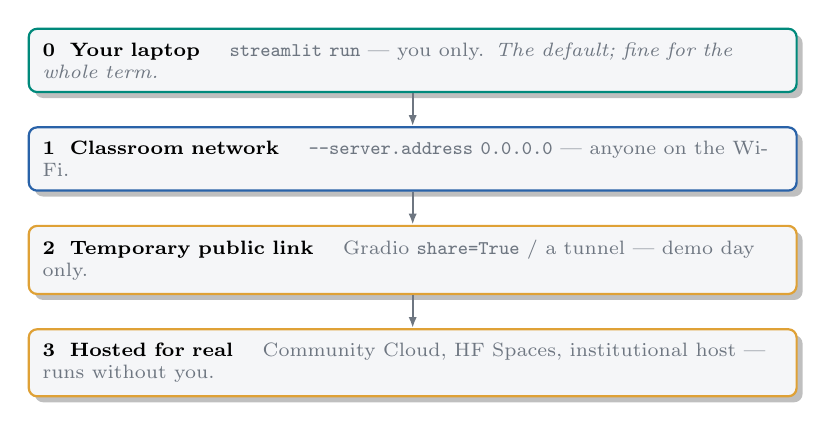
\begin{tikzpicture}[font=\scriptsize, node distance=0.42cm,
      s/.style={rectangle, rounded corners=3pt, draw, thick, fill=lightgray,
                drop shadow, align=left, text width=9.4cm, minimum height=0.72cm,
                inner sep=5pt}]
    \node[s, draw=cRAG]                 (r0) {\textbf{0 \ Your laptop} \quad\textcolor{midgray}{\texttt{streamlit run} --- you only. \emph{The default; fine for the whole term.}}};
    \node[s, draw=cAgent, below=of r0]  (r1) {\textbf{1 \ Classroom network} \quad\textcolor{midgray}{\texttt{--server.address 0.0.0.0} --- anyone on the Wi-Fi.}};
    \node[s, draw=cEval,  below=of r1]  (r2) {\textbf{2 \ Temporary public link} \quad\textcolor{midgray}{Gradio \texttt{share=True} / a tunnel --- demo day only.}};
    \node[s, draw=accentgold, below=of r2] (r3) {\textbf{3 \ Hosted for real} \quad\textcolor{midgray}{Community Cloud, HF Spaces, institutional host --- runs without you.}};
    \draw[-{Latex[length=4pt]}, thick, midgray] (r0)--(r1);
    \draw[-{Latex[length=4pt]}, thick, midgray] (r1)--(r2);
    \draw[-{Latex[length=4pt]}, thick, midgray] (r2)--(r3);
  \end{tikzpicture}
  \end{center}
  \vspace{4pt}
  \begin{center}\small\color{labnavy}\bfseries
    Each rung up adds one reachable stranger --- and one problem you now own.\end{center}
\end{frame}

% ---------------------------------------------------------------- the auth wall
\begin{frame}{The wall you will hit: whose key is answering?}
  \begin{columns}[t, totalwidth=\textwidth]
    \begin{column}{0.48\textwidth}
      \begin{featbox}{accentgold}{\faKey\ Your ALCF token is \emph{personal}}
        \scriptsize
        Browser login $\cdot$ expires in \textbf{$\sim$48 h} $\cdot$ billed to \textbf{you}.
        \\[3pt]On rungs 1--3, every visitor's question is spent \textbf{from your account},
        under \textbf{your name} --- and the app dies when the token does.
      \end{featbox}
    \end{column}
    \begin{column}{0.04\textwidth}\end{column}
    \begin{column}{0.48\textwidth}
      \begin{featbox}{cRAG}{\faLock\ The honest answer}
        \scriptsize
        Rung 3 needs a \textbf{service credential}, not your login --- which the ALCF
        student endpoint does not give you.
        \\[3pt]\textbf{Stay on rung 0--1; use rung 2 for the demo.} A permanent public
        bot needs a different backend and a real conversation.
      \end{featbox}
    \end{column}
  \end{columns}
  \vspace{8pt}
  \begin{calloutbox}[labnavy]
    \small\faExclamationTriangle\ Never paste a token into your code or commit it.
    \texttt{share=True} publishes to \textbf{the open internet with no password}. See
    \texttt{DEPLOY.md} for the checklist.
  \end{calloutbox}
\end{frame}

% ---------------------------------------------------------------- the theological turn
\begin{frame}{The turn: who is answerable for what it says?}
  \begin{columns}[t, totalwidth=\textwidth]
    \begin{column}{0.48\textwidth}
      \begin{featbox}{cAgent}{\faGlobe\ Deploying is a pastoral act}
        \scriptsize
        A CLI answers \textbf{you}, who know its limits. A public chatbot answers a
        \textbf{stranger in distress at 2 a.m.} --- who may read it as counsel.
        \\[3pt]\textbf{The same code; a different moral situation.}
      \end{featbox}
    \end{column}
    \begin{column}{0.04\textwidth}\end{column}
    \begin{column}{0.48\textwidth}
      \begin{featbox}{cEval}{\faBalanceScale\ Minimum decencies}
        \scriptsize
        Say \textbf{what corpus} it reads and \textbf{whose canon} that is. Say it is a
        \textbf{student project}, not a pastor. \textbf{Show the sources.} Say what it
        \textbf{will not} do.
      \end{featbox}
    \end{column}
  \end{columns}
  \vspace{8pt}
  \begin{calloutbox}[accentgold]
    \small\faLightbulb\ Polish is a \textbf{truth claim} users can read. The more finished
    your interface looks, the more your disclosure has to work --- accountability should
    rise \textbf{with} usability, not fall behind it.
  \end{calloutbox}
\end{frame}

% ---------------------------------------------------------------- wrap
\begin{frame}{What to take away \& what to do}
  \begin{featbox}{cRAG}{\faCheckCircle\ Three things}
    \small
    \begin{enumerate}
      \item \textbf{Packaging is thin} --- import your system, never re-implement it
      \item \textbf{A good UI shows its work} --- sources under every answer
      \item \textbf{Every rung of deployment adds a person you are answerable to}
    \end{enumerate}
  \end{featbox}
  \vspace{2pt}
  \begin{featbox}{accentblue}{\faLaptopCode\ To do}
    \small
    \begin{itemize}
      \item Get the chatbot running on \textbf{your own corpus} --- retitle it honestly
      \item Add a \textbf{one-line disclosure} in the sidebar: corpus, canon, ``student project''
      \item Bring it to the \textbf{build sprint}; we demo on rung 1 or 2
    \end{itemize}
  \end{featbox}
  \vspace{2pt}
  \begin{center}\small\color{labnavy}\bfseries
    Next: \textbf{evaluation} --- now that it looks convincing, how do you prove it is right?\end{center}
\end{frame}

\end{document}
